\documentclass{beamer}
\mode<presentation>
{
\usetheme{CambridgeUS}
}

\usepackage{polski}
\usepackage[polish]{babel}
\usepackage[T1]{fontenc}
\usepackage[utf8]{inputenc}
\usepackage{amsmath}
\usepackage{amsthm}
\usepackage{amssymb}
\usepackage{amsfonts}
\usepackage{graphicx}
\usepackage{epsfig}
\usepackage{subfig}
\title{ANOM - Analiza średnich.}
\author{Kamila Komar i Marta Sommer}
\date{26.05.14}

\begin{document}

%\emph{multirow}
	\begin{frame}
	\titlepage
	\end{frame}
%___________________________________________________________

\section{O czym będzie mowa?}
      \begin{frame}
	\frametitle{Plan prezentacji}

	\begin{enumerate}

		\item Wprowadzenie
		\pause
		\item ANOM jednoczynnikowa
		\pause
		\item ANOM dla zadanych specyfikacji
		\pause
		\item ANOM wieloczynnikowa

	\end{enumerate}
      \end{frame}

\section{Wstęp}

  \begin{frame}
 W wielu sytuacjach, potrzebujemy zmierzyć się z problemem porównywania średnich w więcej niż dwóch grupach. Do tego właśnie służy ANOM- analiza średnich. Dzięki testowi wprowadzonemu przez E. R. Ott możemy sprawdzić czy i które ze zbioru $c$-średnich różnią się od średniej ogólnej. Zamiast patrzeć na górne i dolne granice przedziału ufności, patrzymy które z $c$-grup średnich wychodzą poza górną i dolną linię decyzji. Każda średnia powyżej linii decyzyjnej górnej, jest uważana za znacznie wyższą od ogólnej. Podobnie, średnie leżące poniżej dolnej granicy są uznawane za znacznie mniejsze od ogólnej średniej.
\end{frame}     

  \begin{frame}
W przypadku testowania pojedynczego odstępstwa $\overline{X_1}=\overline{X_2}$  korzystamy z testu istotności:
% $$ t=\frac{\overline{x_1}-\overline{x_2}}{\sqrt{\frac{\sigma_1^2}{n_1}+\frac{\sigma_2^2}{n_2}}}, $$
$$ t=\frac{\overline{x_1}-\overline{x_2}}{S_{\overline{X_1}-\overline{X_2}}}, $$
  gdzie:
\begin{enumerate}
		\item[] $\overline{X_1},\ \overline{X_2}$- średnie z prób
		\item[] $n_1,\ n_2$- liczności grup
		%\item[] %$ \sigma_1^2,\ \sigma_2^2$ -odchylenia z prób.
		%$S_{X_1-X_2}$-odchylenie z łącznej próby.
	\end{enumerate} 
	Zatem możemy powiedzieć, że dwie próbki różnią się gdy $t>t_{\alpha},$ gdzie $t_{\alpha}$ poziom krytyczny na poziomie istotności $\alpha.$
  \end{frame}

   \begin{frame}
A CO GDY MAMY WIĘCEJ NIŻ DWIE GRUPY?\\

\bigskip

Czyli chcemy testować:
$$H_0:\overline{X_i}=\overline{\overline{X}}, $$
gdzie $\overline{\overline{X}}$- średnia ogólna.\\
%Możemy to przedstawić jako sumowanie równolicznych próbek, ???????????
\end{frame} 

\section{UDL i LDL}

\begin{frame}
Ogólny pomysł to wyznaczenie linii decyzyjnych.\\
Dolną i górną (LDL i UDL) granicę decyzji wyznaczamy ze wzoru:
$$ \overline{\overline{X}} \pm   h_{\alpha,k,v}S\sqrt{\frac{(k-1)}{kn}}, $$
gdzie:
\begin{enumerate}
		\item[] k -- liczba rozważanych próbek
		\item[] n -- liczność grup
		\item[] $ \overline{\overline{X}}$ -- ogólna średnia
		\item[] %$S^2=\frac{1}{c}\left(S_1^2 + S_2^2+\dots+S_c^2\right)$ 
		$S$ -- estymator wariancji.
		\item[] $h_{\alpha,k,v}$ -- krytyczna wartość statystyki Nelsona
		\item[] $v$ -- liczba stopni swobody związana z $S$ ($=k\cdot(n-1)$)
	\end{enumerate} 
Można udowodnić, że $S\sqrt{\frac{(k-1)}{kn}}$ to estymator wariancji $\overline{X_i}-\overline{\overline{X}}.$
\end{frame} 

\subsection{Przykład}
 \begin{frame}
Rozważmy dane opisujące wpływ temperatury na wydajność procesu:\\

\begin{center}
\scalebox{0.9}{
\begin{tabular}{|r|c|c|c|}
\hline 
&\multicolumn{3}{|c|}{Temperatura}\\
\hline
  Dzień& $250^o$ & $300^o$ & $350^o$ \\
  \hline
 Pn& 2,4& 2,6 &3,2 \\
 Wt &2,7 &2,4 & 3,0 \\
 Śr &2,2 &2,8& 3,1 \\
 Czw & 2,5& 2,5&2,8\\
 Pt & 2,0 &2,2 & 2,5 \\
 & & &\\
 Pn& 2,5& 2,7 &2,9 \\
 Wt &2,8 &2,3 & 3,1 \\
 Śr &2,9 &3,1& 3,4 \\
 Czw & 2,4& 2,9&3,2\\
 Pt & 2,1 &2,2 & 2,6 \\
 \hline
\end{tabular}}
\end{center}

\end{frame}

  \begin{frame}
$$n=10,\hspace{1cm} k=3,\hspace{1cm} \overline{\overline{X}}=2.67$$

Tak jak to robiliśmy w ANOVA możemy wyznaczyć estymator odchylenia standardowego: $$S=\hat{ \sigma}=\sqrt{0.0867} $$\\
$$v = 3\cdot (10-1)=27$$
$$\alpha=0.05$$\\

Z tablic dla statystyki Nelsona odczytujemy wartość $h_{0.05,3,27}=2.485$\\
%$2.485=\frac{1}{2}\left( 2.47+2.50\right)$\\

Podstawmy wszystkie wartości do wzoru: 
$$ \overline{\overline{X}} \pm  h_{\alpha,k,v}S\sqrt{\frac{(k-1)}{kn}}, $$
W wyniku otrzymujemy:
$$LDL=2.48\ i \ UDL=2.86$$
\end{frame}

  \begin{frame}
Graficznie, można to przedstawić w następujący sposób: 
\begin{figure}
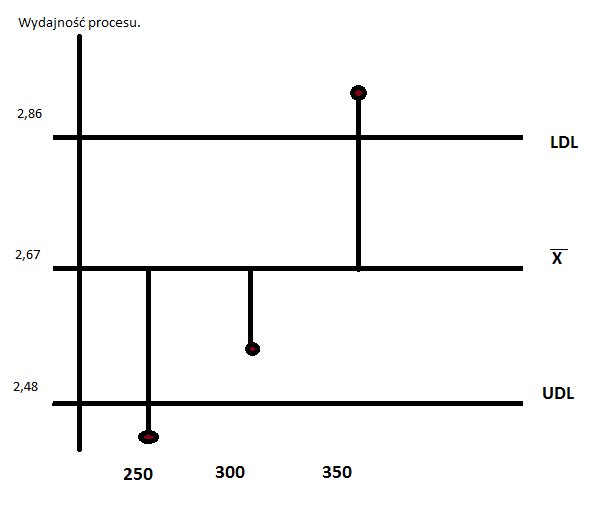
\includegraphics[scale=0.5]{ANOM1.png}
\end{figure}

Widać, że wydajność procesu spada przy $250^\circ$ i jest wyższa niż ogólna średnia przy $350^\circ.$
 
\end{frame}

\subsection{ZAŁOŻENIA}
 \begin{frame}
Założenia, dla tej metody są identyczne jak w przypadku ANOVY:
\begin{enumerate}
		\item[-] niezależność k próbek
		\item[-] normalność rozkładu
		\item[-] jednakowe wariancje
	\end{enumerate} 

\end{frame} 

\section{FRAKCJE}
\subsection{Przykład}
\begin{frame}
Rozważmy dane opisujące firmę (przemysł rolny) zatrudniającą osoby obsługujące kombajny.  Jesteśmy zainteresowani oceną względnej wydajności każdego z pracowników. Rejestrujemy procent upraw nie spełniających specyfikacji, dla każdego pracownika. Chcemy zidentyfikować pracownika, który ma najgorsze wyniki, aby go przeszkolić na nowo lub zwolnić.

\bigskip

Firma zatrudnia 20 pracowników.\\
\end{frame}

\begin{frame}
\begin{center}
\scalebox{0.9}{
\begin{tabular}{|c|c|}
\hline 
  Numer pracownika & Niezgodność upraw (\%) [n=1000] \\
  \hline
$1$& $1,4$\\
$2$&  $2,6$\\
$3$& $1,0$  \\
$4$&  $3,1$\\
$5$&  $2,9$\\
$6$& $5,1$ \\
$7$&  $2,4$\\
$8$&  $4,1$\\
$9$& $1,1$\\
$10$& $2,1$\\
$11$& $2,0$\\
$12$& $2,6$\\
$13$& $3,1$\\
$14$& $2,7$\\
$15$& $\cdots$\\

 \hline
\end{tabular}}
\end{center}
\end{frame} 

\begin{frame}
W przypadku takich danych linie decyzyjne wyznaczamy ze wzoru:
$$ \overline{p}\hspace{5mm} \pm\hspace{5mm} h_{\alpha,k,\infty}\cdot S_p\cdot\sqrt{\frac{k-1}{k}},$$
gdzie: 
\begin{enumerate}
		\item[] $\overline{p}$ -- średnia ze wszystkich proporcji %tu 20
		\item[] $S_p=\sqrt{\frac{\overline{p}\left(1-\overline{p}  \right)}{n}}$ -- estymator $\sigma_p$
		\item[] k -- liczba grup
	\end{enumerate} 
\end{frame}

\begin{frame}
W przypadku wspomnianych danych mamy:
$$\overline{p}=0.02775 $$
$$S_p=\sqrt{\frac{0.02775\cdot 0.97225}{1000}}=0.0052   $$
$$k=20$$
Z tabeli wartości statystyki Nelsona odczytujemy wartość: $$h_{0.05,20,\infty}=3.02.$$
W praktyce częściej przyjmuje się poziom istotności $\alpha=0.01$  i wtedy
$$h_{0.01,20,\infty}=3.48.$$
%aby mowic pracownikowi mniej razy ze probka jest zla, jesli faktycznie byla dobra
W ten sposób otrzymaliśmy $$LDL=0,0101\ i\ UDL=0.0454$$
\end{frame}

\begin{frame}
Nasze wyniki przedstawione graficznie:
\begin{figure}
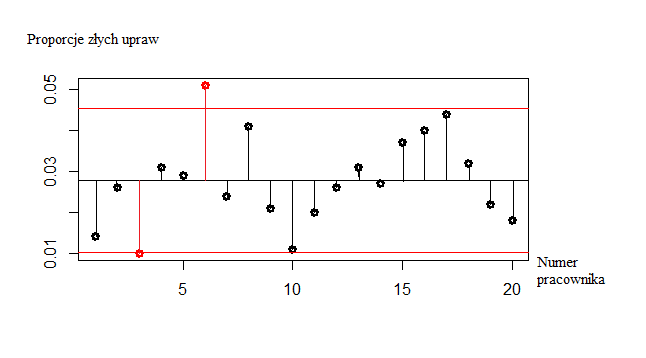
\includegraphics[scale=0.5]{ANOM2.png}
\end{figure}
Z powyższej postaci graficznej od razu widać, że mamy 11 obserwacji powyżej średniej i 9 poniżej. Ponadto wynik obserwowany dla pracownika o numerze 6 przekracza UDL. Pracownik nr. 3 ma wynik leżący poniżej LDL oraz pracownik 9 bardzo zbliża się do niej.
\end{frame}

%\subsubsection{FAKTY}
%\begin{frame}
%Warto jeszcze zwrócić uwagę na fakt, że takie użycie metody ANOM dla proporcji może być alternatywą dla testu zgodności %$\chi^2.$\\
%%tzn moglibysmy badac w tym przypadku rownosc 20proporcji
%ANOM jest bardziej wrażliwa na wykrywanie kilku ekstremalnych odchyleń od średniej.\\
%Niezbędnym założeniem ANOM dla proporcji jest założenie o asymptotycznej normalności rozkładu dwumianowego. Jeśli mamy %wątpliwość , co do adekwatności aproksymacji, to powinniśmy dokonać przekształceń danych.
%\end{frame}

\section{DANE DYSKRETNE}
\subsection{Przykład}
\begin{frame}
ANOM możemy używać, gdy mamy odczynienia z danymi dyskretnymi, które powinny być opisywane rozkładem Poissona. Linie decyzyjne w tym przypadku wyznacza się ze wzoru:
$$\overline{c} \pm h_{\alpha,k,\infty}\cdot\sqrt{\overline{c}}\cdot\sqrt{\frac{k-1}{k}},  $$
gdzie: 
\begin{enumerate}
		\item[] $\overline{c}$ - średnia z $k-$zliczeń 

	\end{enumerate} 
Możliwość użycia ANOM w tym przypadku opiera się na założeniu aproksymacji rozkładu Poissona do rozkładu normalnego. Jeśli dane nie spełniają założeń, należy dokonać ich transformacji.
\end{frame}

%%%%%%%%%%%%%%%%%%%%%%%%%%%%%%%%%%%%%%%%%%%%%%%%%%%%%%%%%%%%%%%%%%%%%%%%%%%%%%%%%%%%%%%%%%%%%%%%%%%%%%%%%%%%%%%%%%%%%%
%%%%%%%%%%%%%%%%%%%%%%%%%%%%%%%%%%%% MARTA %%%%%%%%%%%%%%%%%%%%%%%%%%%%%%%%%%%%%%%%%%%%%%%%%%%%%%%%%%%%%%%%%%%%%%%%%%%
%%%%%%%%%%%%%%%%%%%%%%%%%%%%%%%%%%%%%%%%%%%%%%%%%%%%%%%%%%%%%%%%%%%%%%%%%%%%%%%%%%%%%%%%%%%%%%%%%%%%%%%%%%%%%%%%%%%%%%

\begin{frame}
\frametitle{ANOM przy zadanych standardach}
Dla proporcji:
$$
p\hspace{2mm}\pm\hspace{2mm}h_{\alpha,k,\infty}\cdot\sqrt{\dfrac{p(1-p)}{n}}
$$
Dla danych dyskretnych:
$$
c\hspace{2mm}\pm\hspace{2mm}h_{\alpha,k,\infty}\cdot\sqrt{c}
$$
\end{frame}

\begin{frame}
\frametitle{ANOM przy zadanych standardach}
Dla danych liczbowych ($\sigma$ i $\mu$ znane):
$$
\mu\hspace{2mm}\pm\hspace{2mm}h_{\alpha,k,\infty}\cdot\dfrac{\sigma}{\sqrt{n}}
$$
Dla danych liczbowych ($\mu$ jest nieznane, a $\sigma$ jest znane):
$$
\overline{\overline{x}}\hspace{2mm}\pm\hspace{2mm}h_{\alpha,k,\infty}\cdot\dfrac{\sigma}{\sqrt{n}}\cdot\sqrt{\dfrac{k-1}{k}}
$$
Dla danych liczbowych ($\mu$ jest znane, a $\sigma$ jest nieznane):
$$
\mu\hspace{2mm}\pm\hspace{2mm}h_{\alpha,k,\nu}\cdot\dfrac{S}{\sqrt{n}}
$$
\end{frame}

\begin{frame}
\frametitle{ANOM wieloczynnikowa}
Efekt A i B. 

\bigskip

Linie kontrolne dla efektów A i B wyznaczamy standardowo ze wzoru:
$$
\overline{\overline{x}}\hspace{2mm}\pm\hspace{2mm}h_{\alpha,k,\infty}\cdot\dfrac{S}{\sqrt{n}}\cdot\sqrt{\dfrac{k-1}{k}}
$$

\bigskip

Ale należałoby też uwzględnić integracje!
\end{frame}

\begin{frame}
\frametitle{Interakcje}
Interakcje wyznaczamy z następującego wzoru:
$$
\overline{L}=\dfrac{1}{2}(\overline{A_1B_1}+\overline{A_2B_2})
$$
$$
\overline{U}=\dfrac{1}{2}(\overline{A_1B_2}+\overline{A_2B_1})
$$
Wtedy:
$$
AB = \overline{L} - \overline{U}
$$

\bigskip

Linie decyzyjne dla AB wyznaczane są z tego samego wzoru, co dla A i B.
\end{frame}

\begin{frame}
\frametitle{Rysunek}
\begin{center}
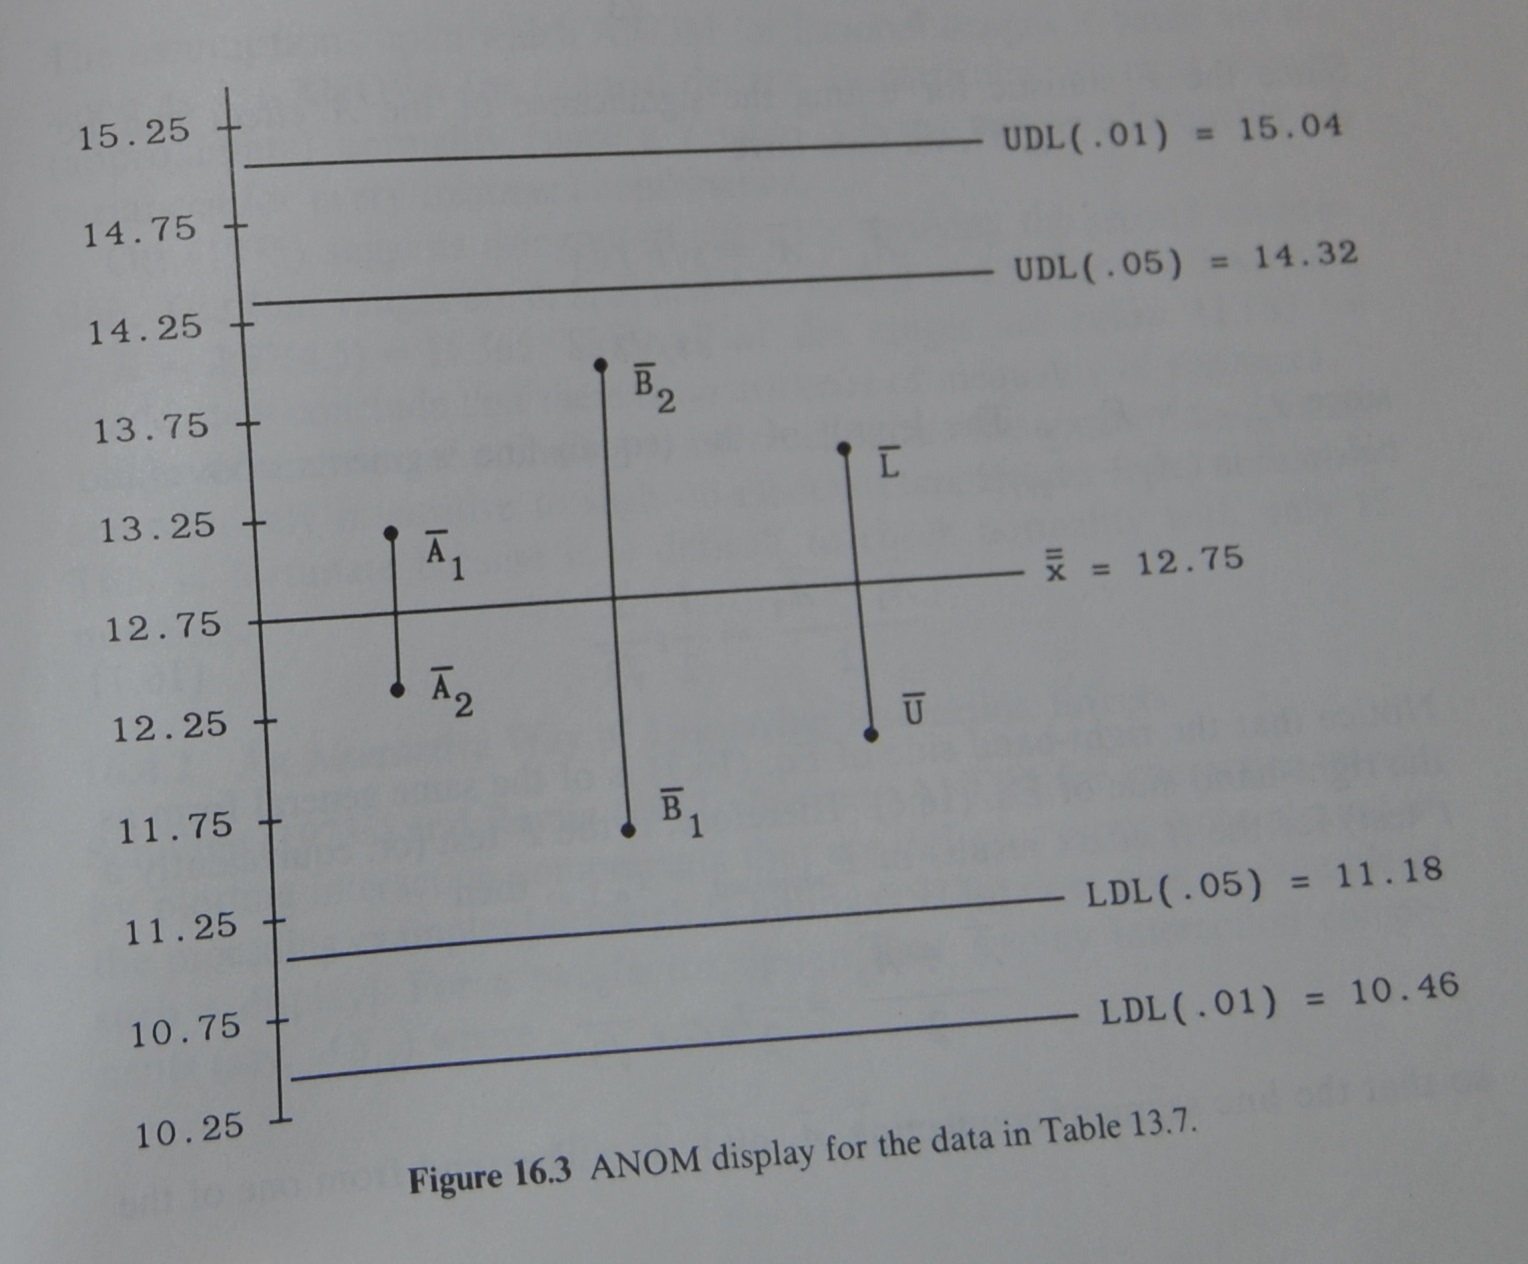
\includegraphics[scale=0.7]{in.jpg}
\end{center}
\end{frame}

\begin{frame}
\frametitle{Inny sposób wyznaczania interakcji}
$$
AB_{ij} =  \overline{AB_{ij}} - \overline{A_{i}} - \overline{B_{j}} + \overline{\overline{x}}
$$

\bigskip

Problemy:

\begin{enumerate}

\item[] -- inna skala rysunku niż dla średnich w grupach
\item[] -- nie znamy wartości $h_\alpha$ dla takiej statystyki

\end{enumerate}
\end{frame}

\begin{frame}
\frametitle{ANOM wieloczynnikowa, przy wielu poziomach czynnika}
\begin{center}
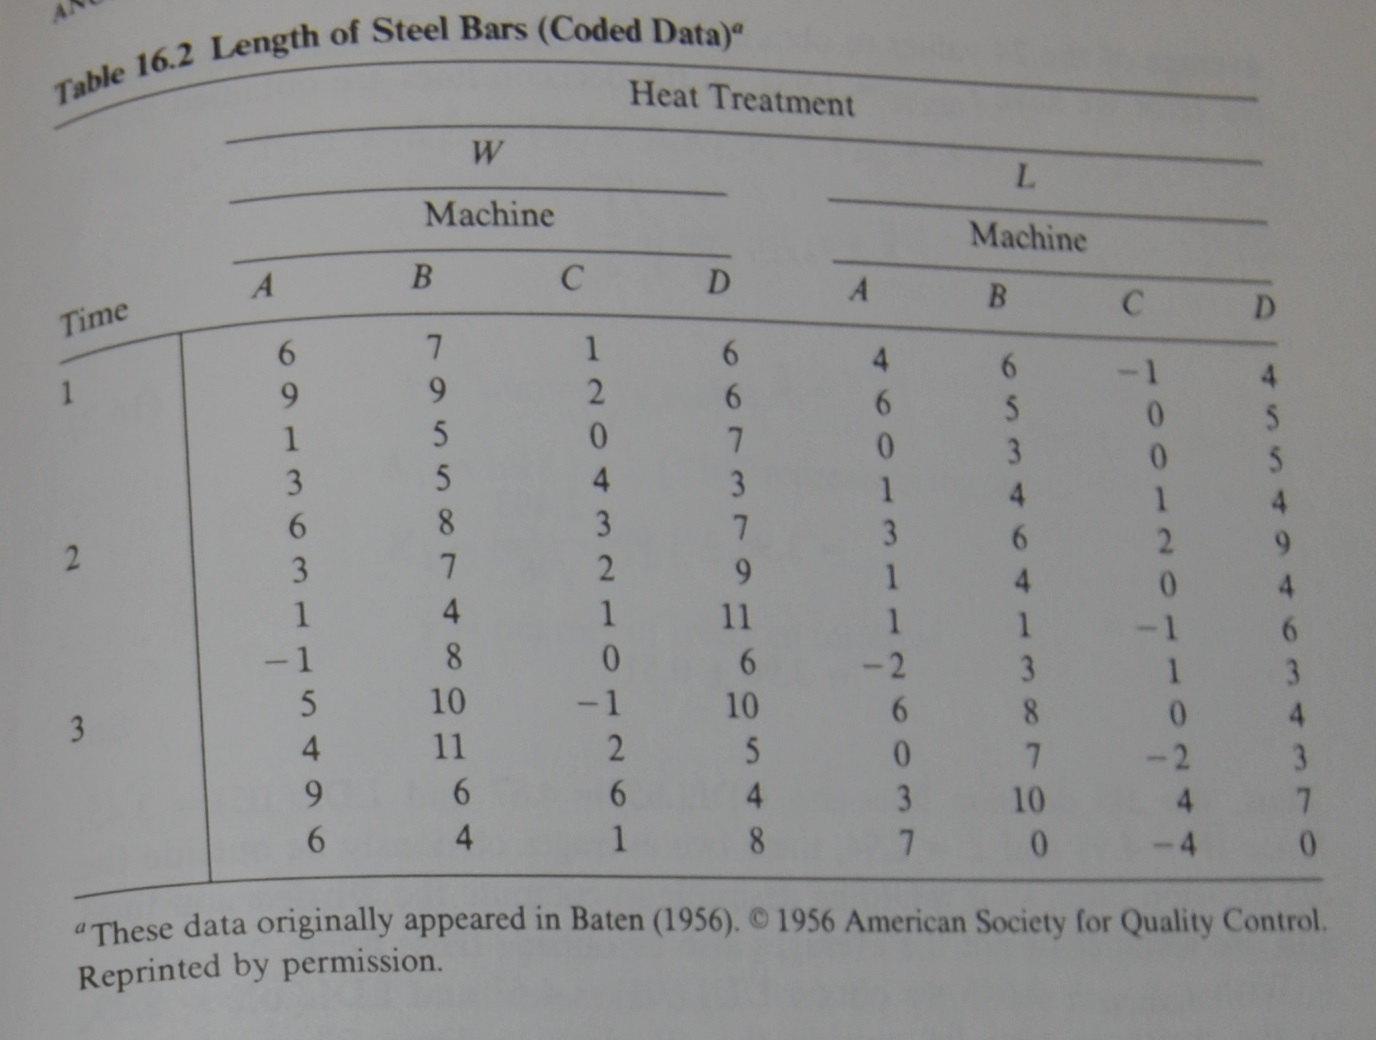
\includegraphics[scale=0.9]{tab.jpg}
\end{center}
\end{frame}

\begin{frame}
\frametitle{ANOM wieloczynnikowa, przy wielu poziomach czynnika}

Stosujemy po prostu do każdego czynnika zwykłą ANOM.

\bigskip

Tak więc:
$$
\overline{T_1} = 3,78, \hspace{5mm} \overline{T_2} = 3,625, \hspace{5mm} \overline{T_3} = 4,47
$$
$$
\overline{W} = 4,98, \hspace{5mm} \overline{L} = 2,94
$$
$$
\overline{A} = 3,42, \hspace{5mm} \overline{B} = 5,875, \hspace{5mm} \overline{C} = 0,875 \hspace{5mm}, \overline{D} = 5,67
$$
$$
\overline{\overline{x}} = 3,96
$$

\end{frame}

\begin{frame}
\frametitle{ANOM wieloczynnikowa, przy wielu poziomach czynnika}
\begin{center}
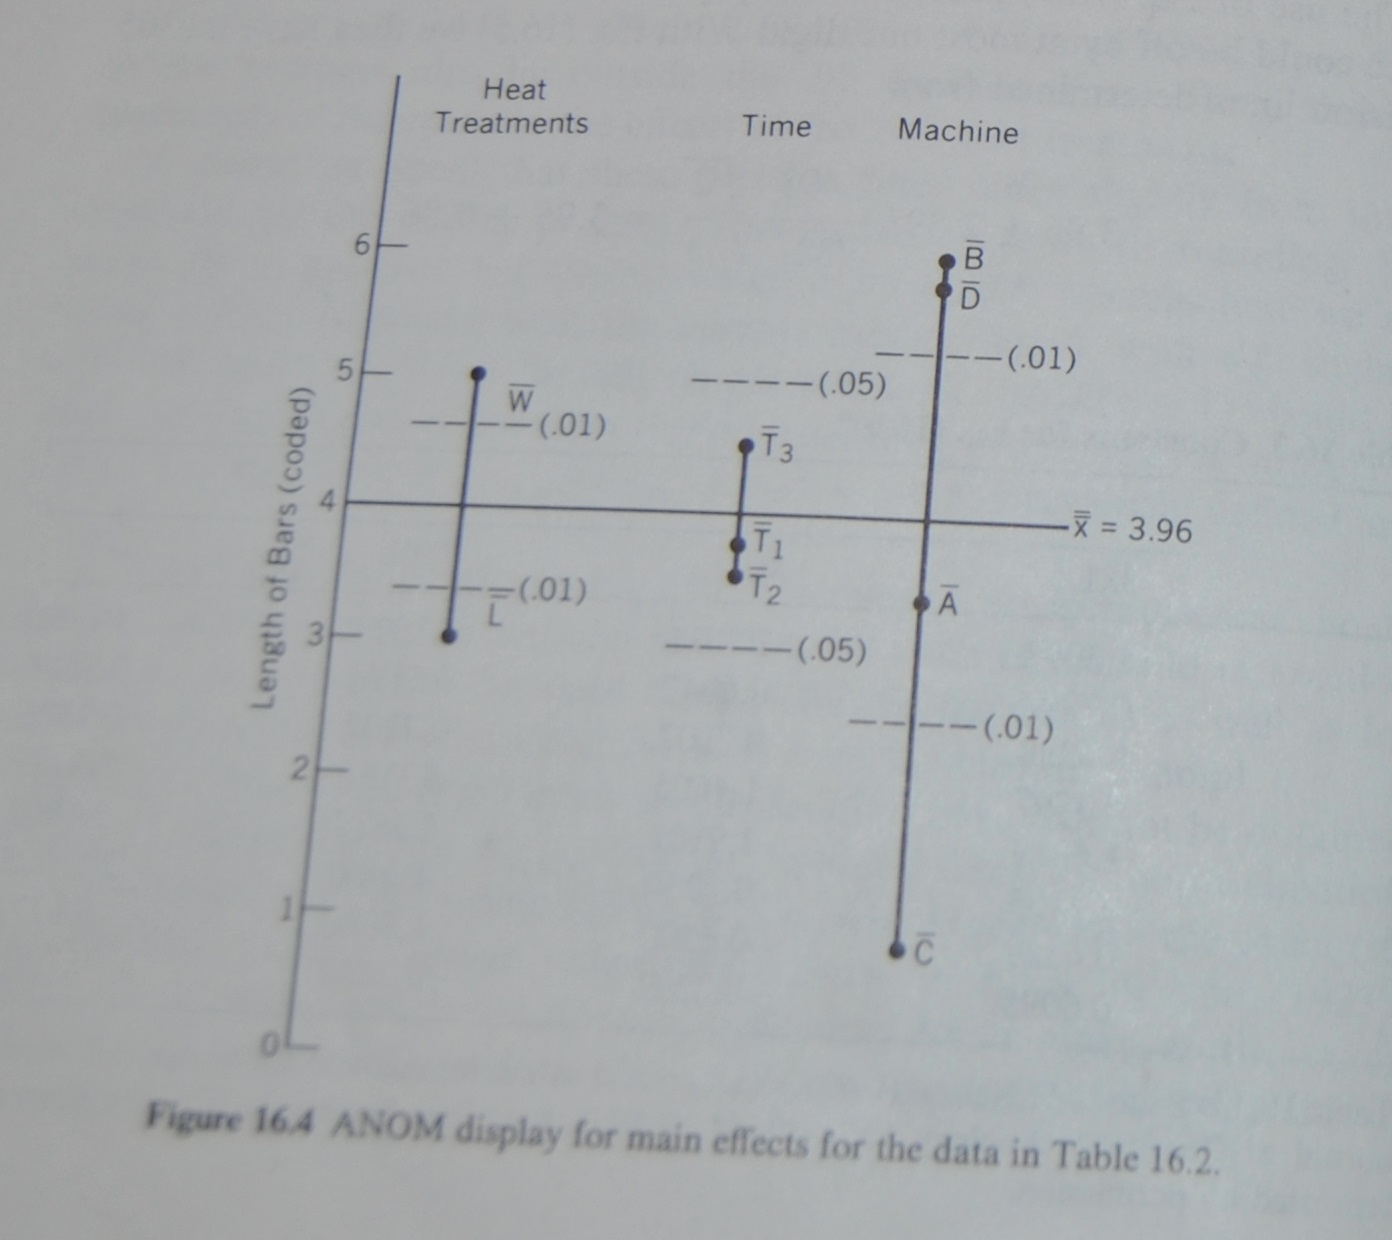
\includegraphics[scale=0.8]{w.jpg}
\end{center}
\end{frame}


%%%%%%%%%%%%%%%%%%%%%%%%%%%%%%%%%%%%%%%%%%%%%%%%%%%%%%%%%%%%%%%%%%%%%%%%%%%%%%%%%%%%%%%%%%%%%%%%%%%%%%%%%%%%%%%%%%%%%%%
\begin{frame}
\frametitle{BIBLIOGRAFIA}
\begin{thebibliography}{99}
\bibitem{pa} Thomas P. Ryan 
\emph{Statistical Methods for Quality Improvement},\\ WILEY (1989), rozdział 16.

\end{thebibliography}
\end{frame}

	%______________________________________________________________________________
\section{!!!!!!!!}	
	\begin{frame}
\frametitle{;)}
\center \Huge{\textsl{\textbf{DZIĘKUJEMY!}}}\\
\end{frame}	

\end{document}